\section{Evaluation}
What do we need, what do we have, what is best suited so far?

Using unsupervised features for action recognition is still in its beginning but promising.
The amount of research that has been put into supervised methods, i.e.\ 3d convnets two-stream approaches can boost unsupervised methods when done there.
Big advantage: no labeling, or less labeling needed when using semi-supervised learning.
Amount of video on the internet huge -> potential.

table conventional:
TODO

table deep:\\
\cite{ji_3d_2013}\\
\cite{baccouche_sequential_2011}\\
\cite{karpathy_large-scale_2014}\\
\cite{tran_learning_2015}\\
\cite{varol_long-term_2016}\\
\cite{simonyan_two-stream_2014}\\
\cite{ng_beyond_2015}\\
\cite{wang_towards_2015}\\
\cite{feichtenhofer_convolutional_2016}\\
\cite{wang_action_2015}\\
\cite{srivastava_unsupervised_2015}\\

\begin{table}[H]
    \centering
    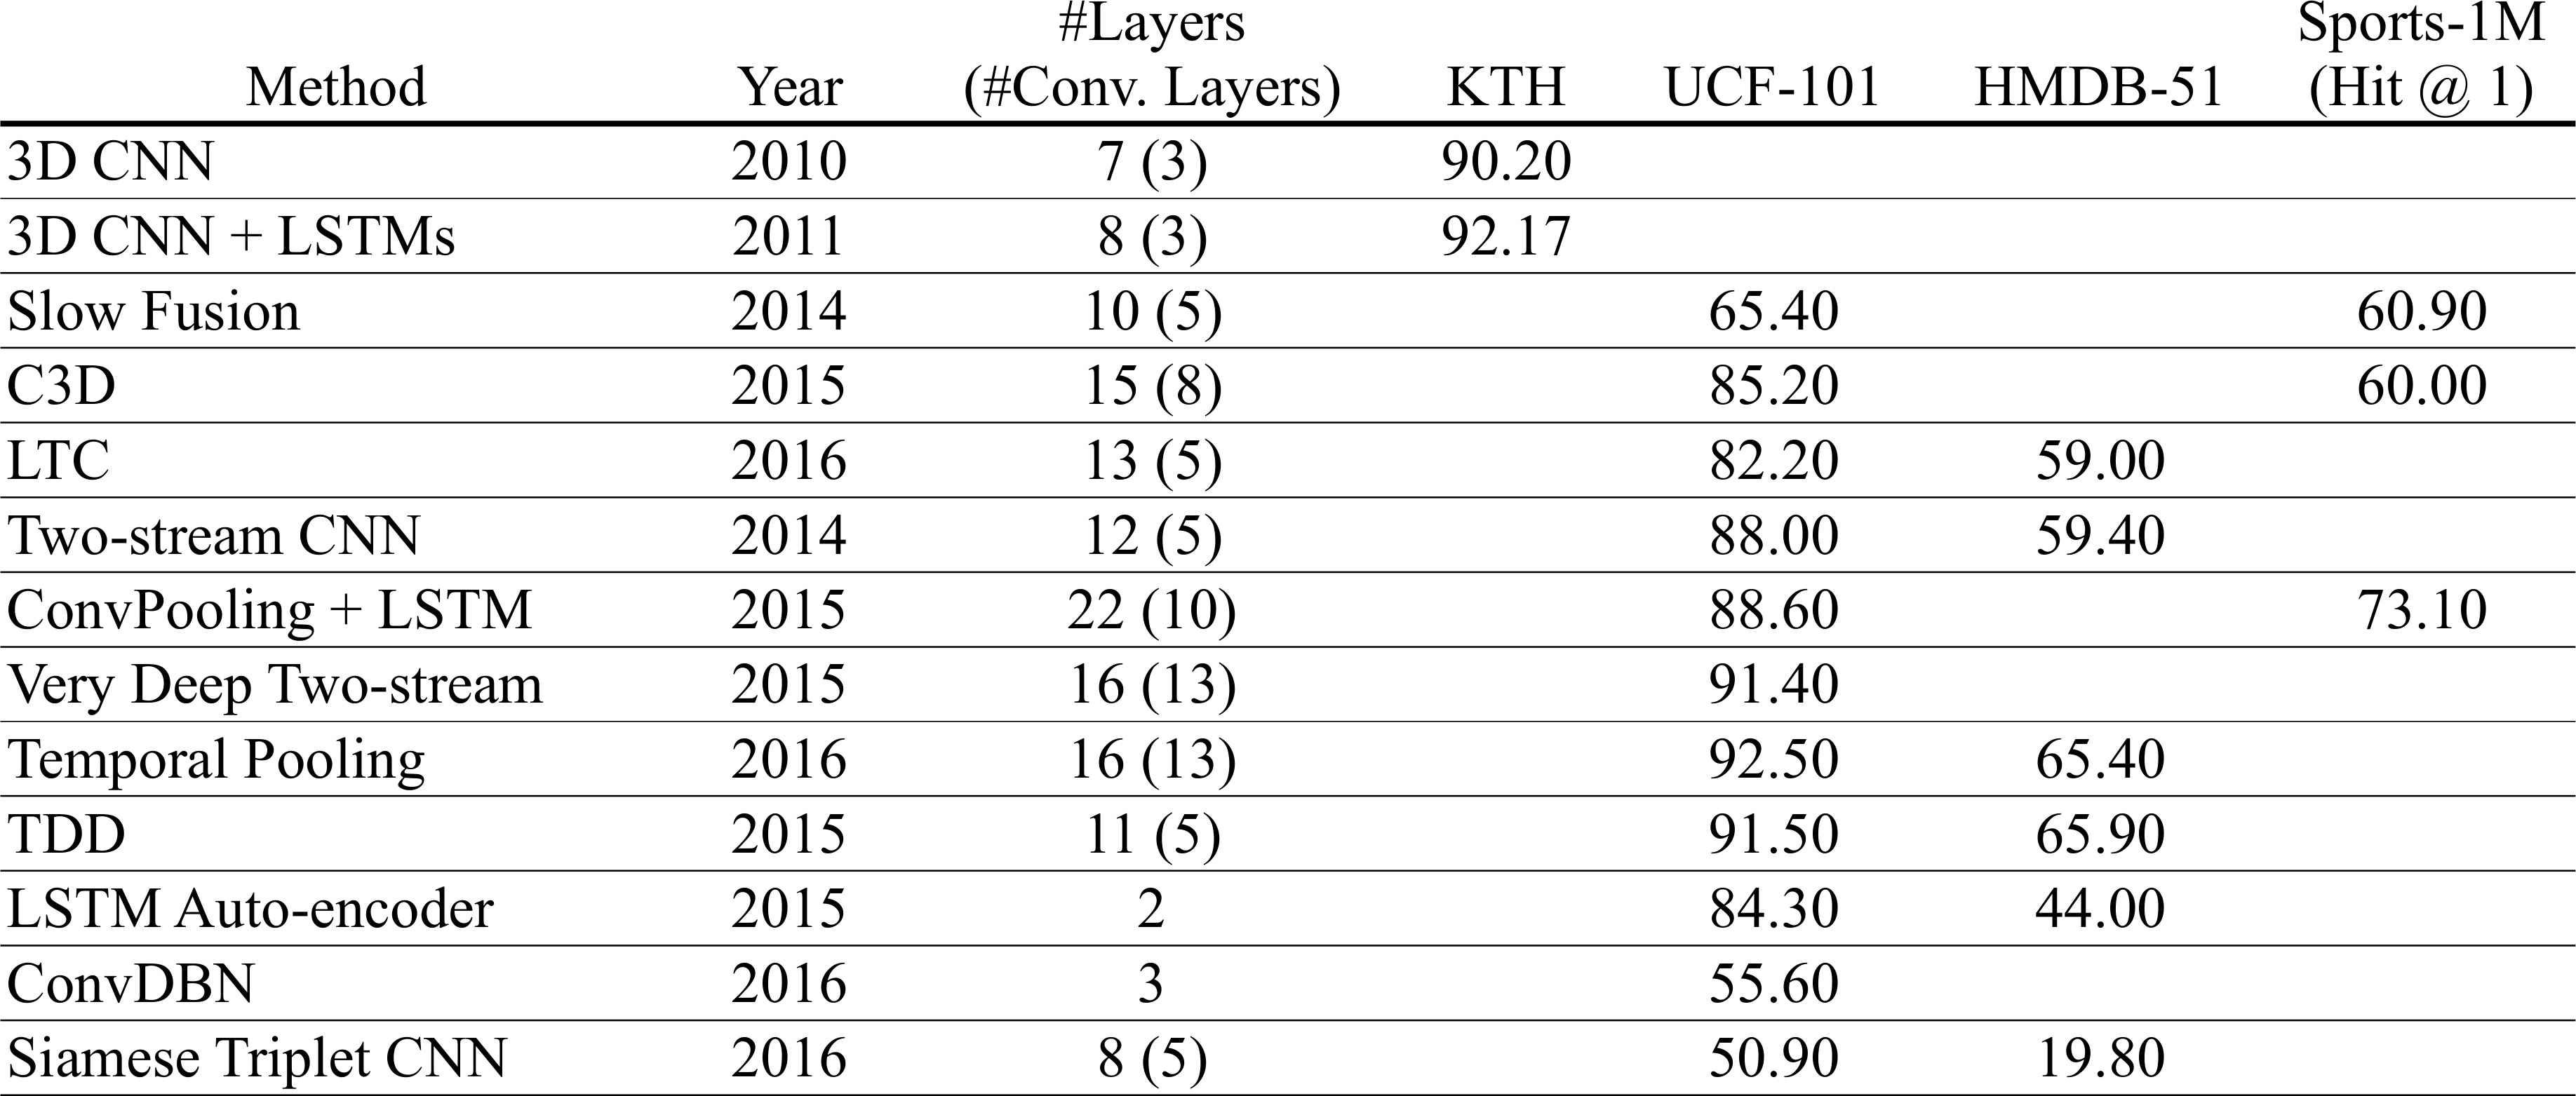
\includegraphics[width=\textwidth]{img_evaluation/deep_results}
    \caption{Best reported action recognition accuracies of reviewed deep learning approaches.}
    \label{tab:deep_results}
\end{table}

table datasets:
\begin{table}
    \centering
    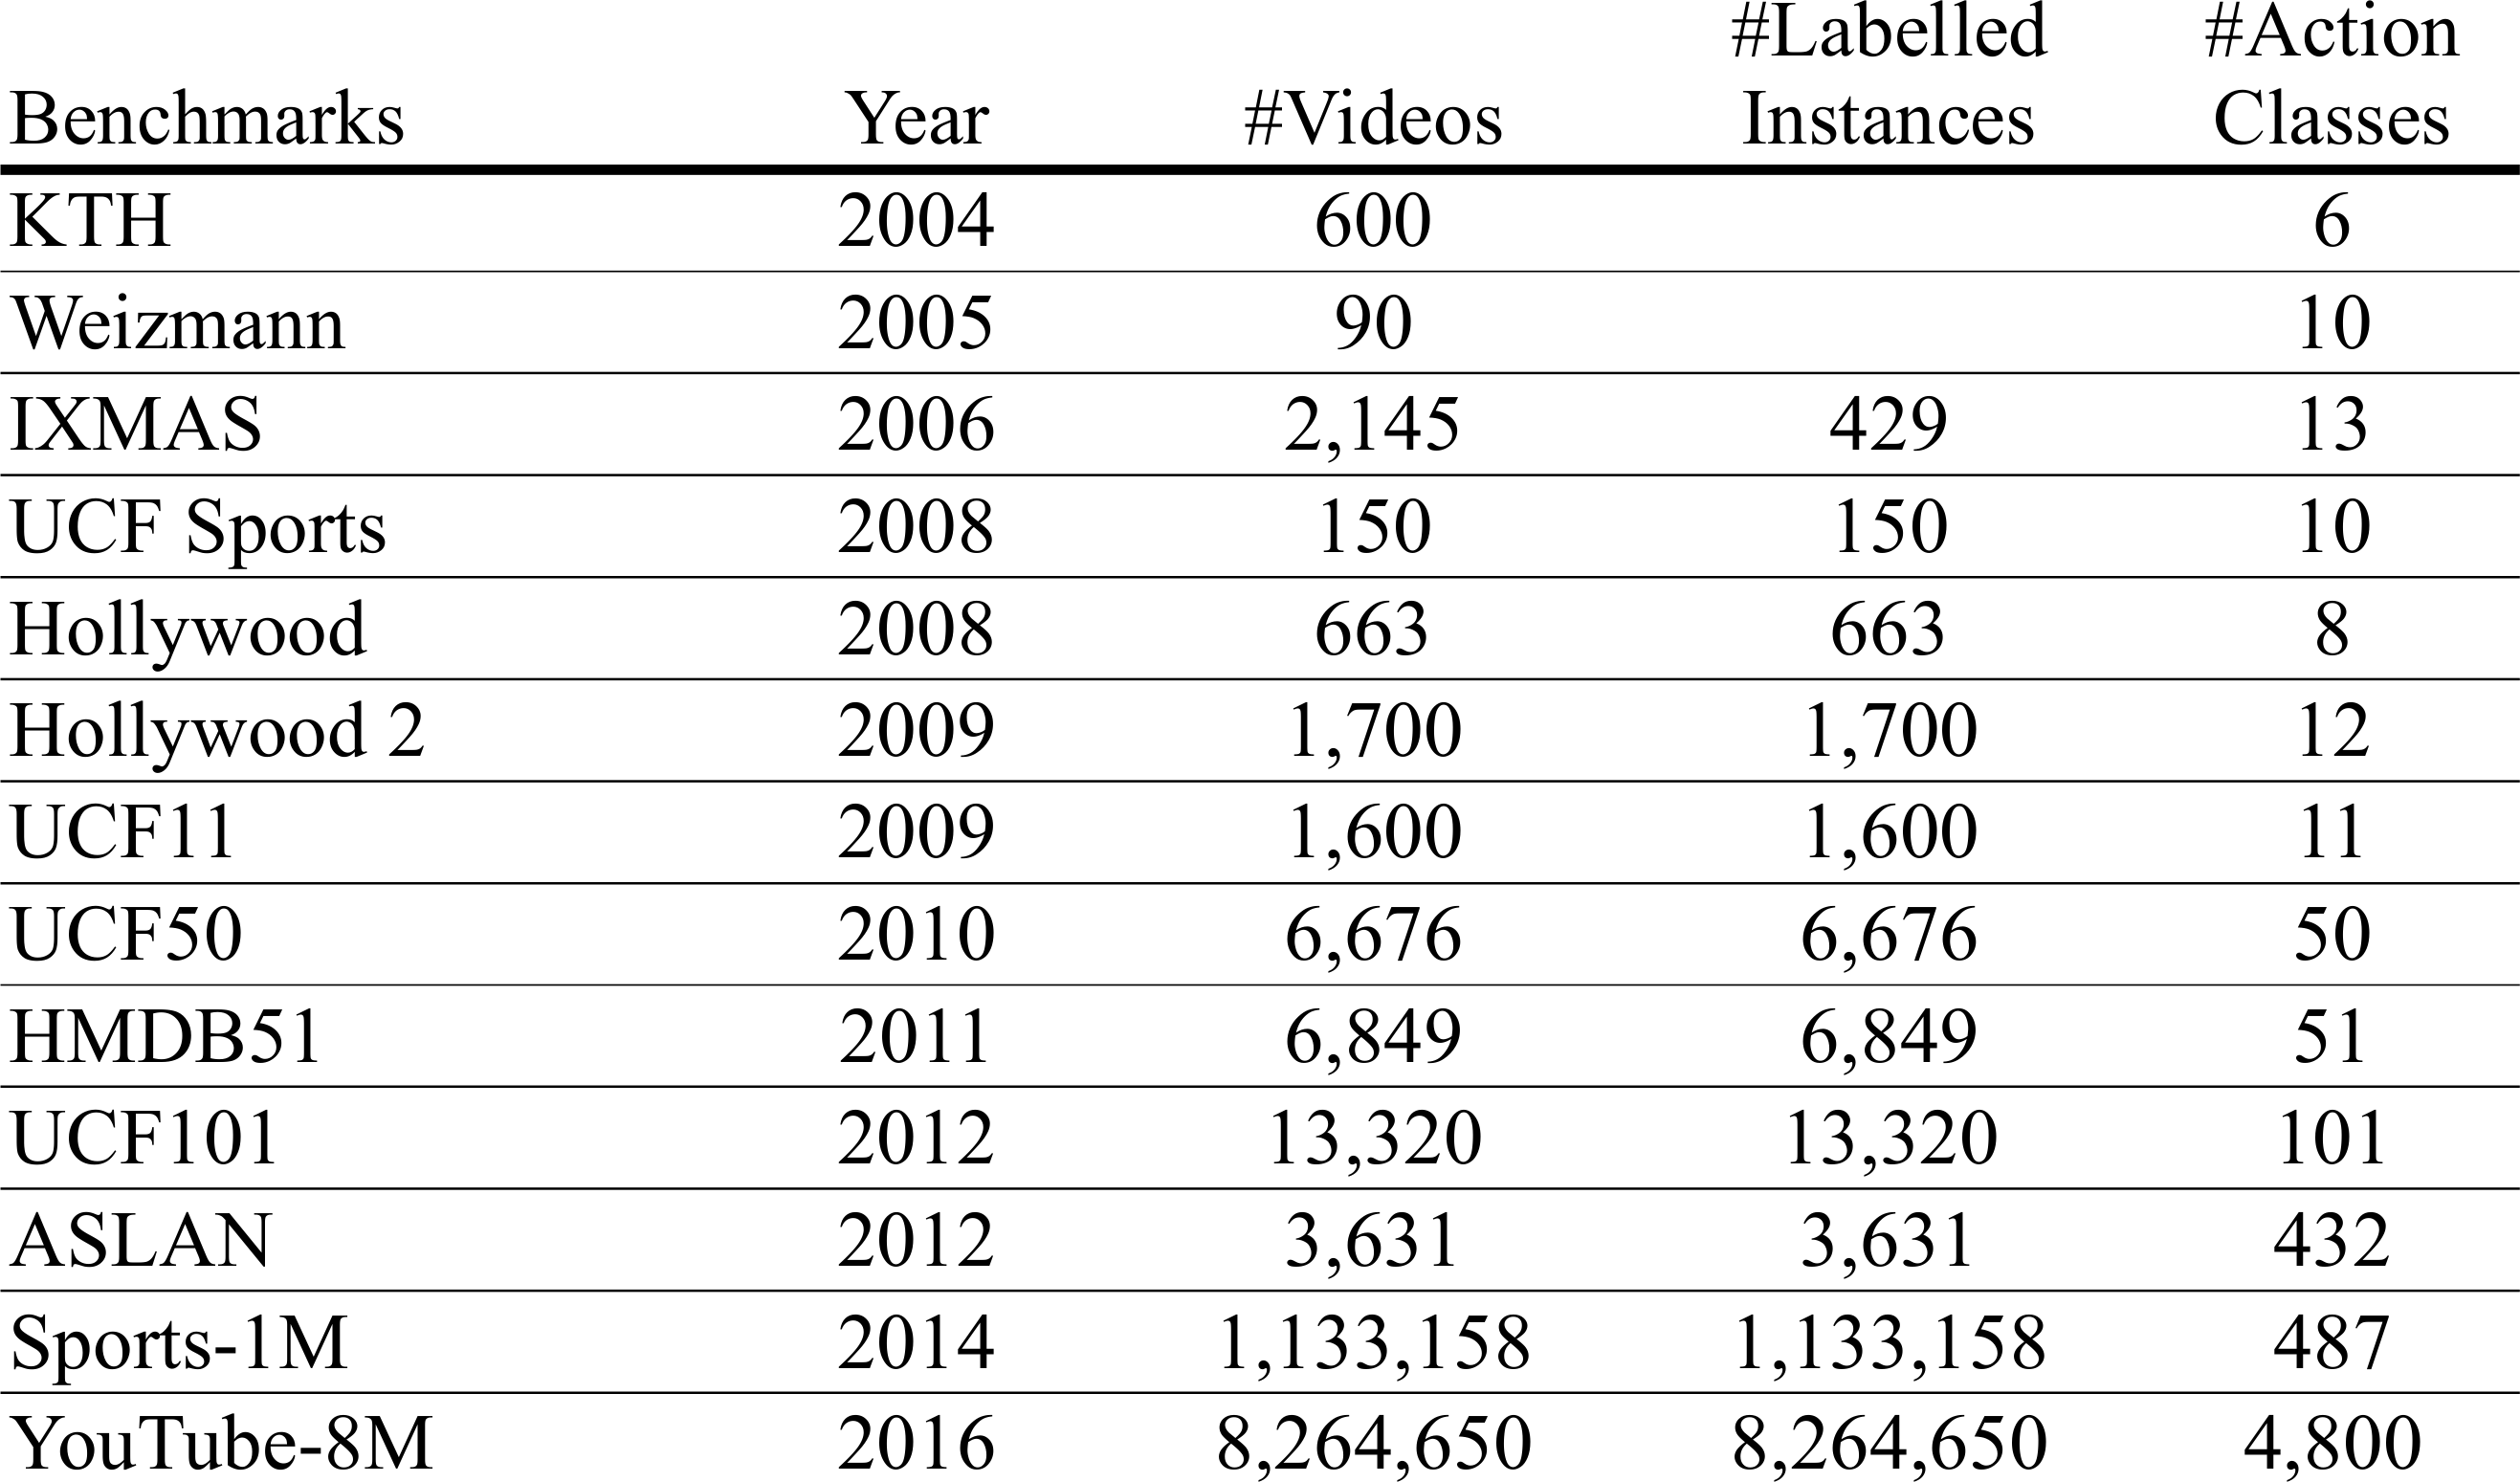
\includegraphics[width=0.7\textwidth]{img_evaluation/benchmarks_results}
    \caption{Size comparison of reviewed benchmarking datasets}
    \label{tab:benchmarks_results}
\end{table}

\begin{table}
    \centering
    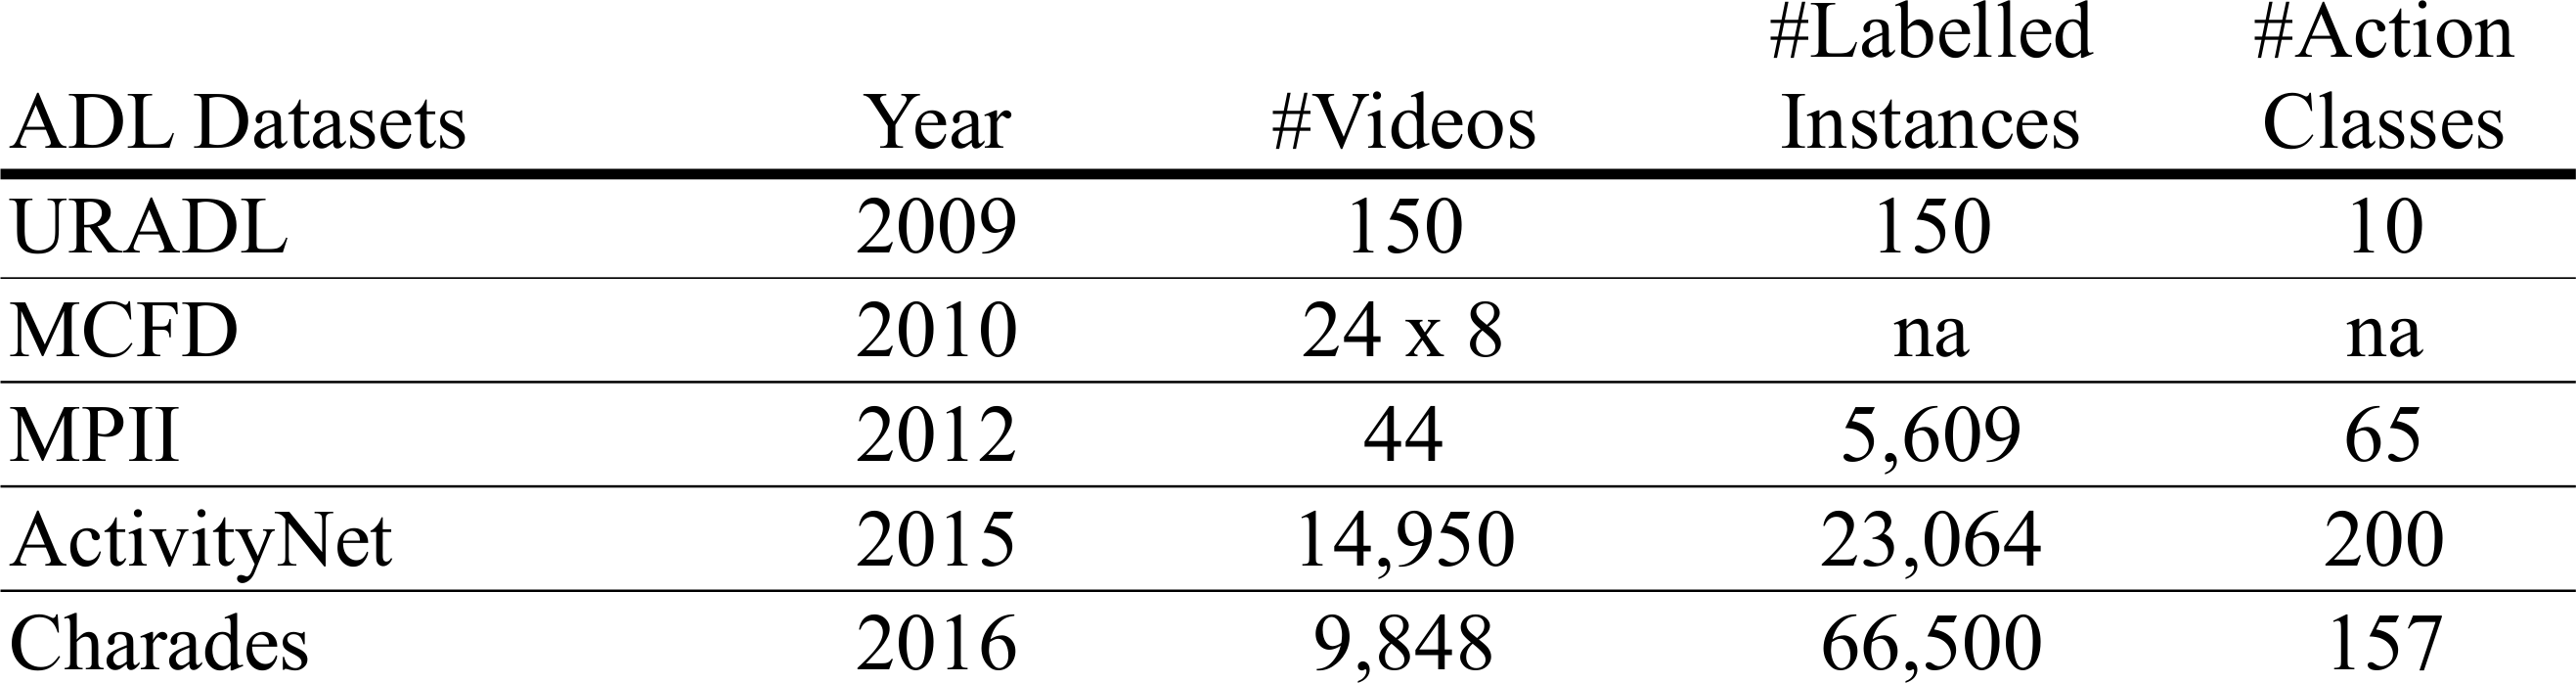
\includegraphics[width=0.7\textwidth]{img_evaluation/adl_results}
    \caption{Size comparison of reviewed daily-living datasets}
    \label{tab:adl_results}
\end{table}


code available: feichtenhofer

see table in ``towards good practices'' (conventional methods state-of-the-art)

available code for C3D and ``towards good practices''

future directions: transfer learning, as done by karpathy, large scale
pre-training, as done by varol et. al 2016
multi task learning as done by two stream approach simonyan and zisserman

future directions: integrating recurrent structure directly into CNNs 

datasets too small. Citation: karpathy, large-scale classification: ``From a practical standpoint, there are currently no video classification benchmarks that match the scale and variety of existing image datasets because videos are significantly more difficult to collect, annotate and store.''

datasets too small. citation: simonyan zisserman ``Unlike the spatial stream ConvNet, which can be pre-trained on a large still image classification dataset (such as ImageNet), the temporal ConvNet needs to be trained on video data – and the available datasets for video action classification are still rather small''.

datasets too small, architectures too shallow \cite{wang_towards_2015}

Due to the label noise, learning spatiotemporal ConvNets still largely relies on smaller, but temporally consistent datasets such as UCF101 [24] or HMDB51 [13] which contain short videos of actions.
This facilitates learning, but comes with the risk of severe overfitting to the training data. Feichtenhofer 2016

UCF101 is considered extremely small. cite Towards good practices for very deep two-stream ConvNets -- wang 2015.

``From a practical standpoint, there are currently no video classification benchmarks that match the scale and variety of existing image datasets because videos are significantly more difficult to collect, annotate and store.'' cite large-scale image classification

``In particular, commonly used datasets (KTH, Weizmann, UCF Sports, IXMAS, Hollywood 2, UCF-50) only contain up to few thousand clips and up to few dozen classes.
Even the largest available datasets such as CCV (9,317 videos and 20 classes) and the recently introduced UCF-101[22] (13,320 videos and 101 classes) are still dwarfed by available image datasets in the number of instances and their variety [7].'' cite large-scale image classification

``Extensions of CNNs to action recognition in video have been proposed in several recent works [6, 12, 13]. Such methods, however, currently show only moderate improvements over earlier methods using hand-crafted video features [5].''
Varol Long term temporal convolutions.

Most of the current CNN methods use architectures with 2D convolutions, enabling shift-invariant representations in the image plane. Meanwhile, the invariance to translations in time is also important for action recognition since the beginning and the end of actions is unknown in general. Laptev 2016

improved trajectories identified as state-of-the-art approach. cite simonyan and zisserman ``There still remain some essential ingredients of the state-of-the-art shallow representation [26], which are missed in our current architecture''

\subsection{Comparison Deep Learning Methods}
Nice comparison in related work section of ``Beyond Temporal Pooling:  Recurrence and Temporal Convolutions for Gesture Recognition in Video''
Convolutions for Gesture Recognition in Video

One problem of deep learning methods is that they require a large number of labeled videos for training, while most available datasets are relatively small.
Meanwhile, most of current deep learning based action recognition methods largely ignore the intrinsic difference between temporal domain and spatial domain, and just treat temporal dimension as feature channels when adapting the architectures of ConvNets to model videos.

Introduction of Feichtenhofer: Current state of the art - Tran and TDD.

\subsection{Data Augmentation Methods}

refer to Imagenet classification with deep convolutional neural networks.

RGB colour Jittering

the improved data augmentation scheme (different aspect-ratio, fixed crops)
from [61] for all our methods and baselines.
61: Wang, L., Xiong, Y., Wang, Z., Qiao, Y.: Towards good practices for very
deep two-stream convnets. arXiv preprint arXiv:1507.02159 (2015)

\subsection{Inter-Dataset Approaches}
META: A.k.a methods to relax the need for large dataset sizes

\subsubsection{Unsupervised pre-training}

\subsubsection{Multi-task learning}

\subsubsection{Transfer learning}

See Karparthy 'Large-scale video classification with convolutional neural networks' 2014

A. S. Razavian, H. Azizpour, J. Sullivan, and S. Carls-
son. CNN features off-the-shelf: an astounding baseline for
recognition

N. Zhang, M. Paluri, M. Ranzato, T. Darrell, and L. Bourdev. Panda: Pose aligned networks for deep attribute modeling. In CVPR, 2014.

B. Zhou, A. Lapedriza, J. Xiao, A. Torralba, and A. Oliva. Learning deep features for scene recognition using places database. In NIPS, 2014.
